\section{Struttura simplettica del fibrato cotangente}
\setcounter{equation}{0}

Sia $M$ una varietà differenziabile (che poi identificheremo con $\mathcal{V}_{n+1}$) e che riferiremo per generalità e semplicità a coordinate locali $x^1, \dots , x^m$.
\begin{multicols}{2}
%\smallskip
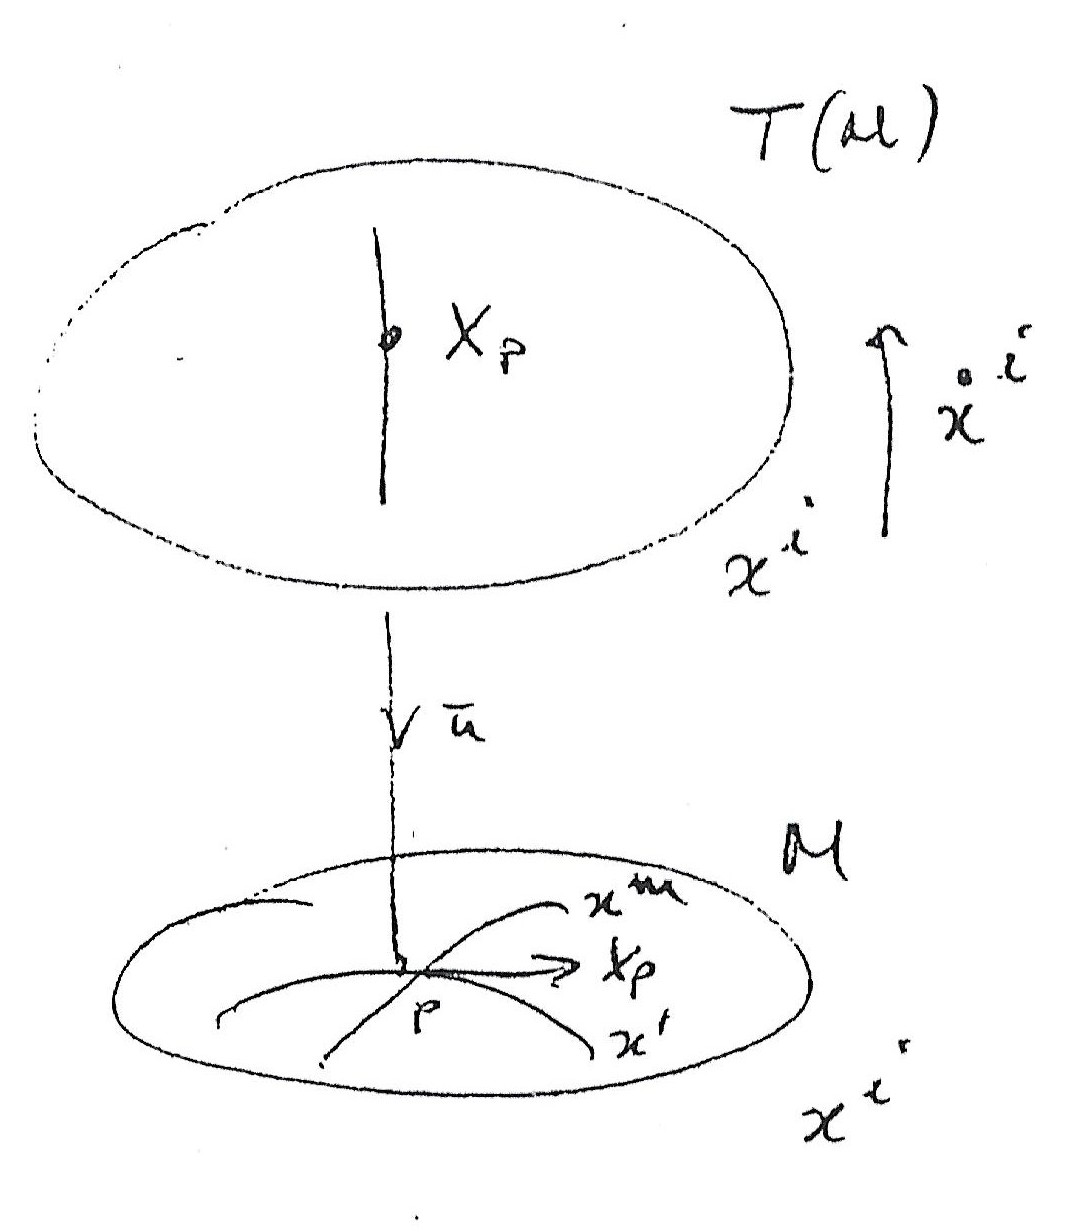
\includegraphics[width=\columnwidth]{media/struttura-simplettica-del-fibrato-cotangente/20-1}
\begin{equation*}
X_p = (X_P)^i \frac{\partial}{\partial x^i} \overset{def}{=} \dot{x}_P^i \bigg( \frac{\partial}{\partial x^i} \bigg)_P
\end{equation*}
$T(M) =$ spazio (fibrato su $M$) costituito dalla totalità dei \textit{vettori} applicati in tutti i punti di $M$
\\
$x^i, ~\dot{x}^i$ \quad coordinate \textit{naturali} su $T (M)$ \\
\begin{equation*}
X_P = \dot{x}_P^i \frac{\partial}{\partial x^i} = \dot{x}_P^i \frac{\partial x'^k}{\partial x^i}\frac{\partial}{\partial x'^k} 
\end{equation*}
\begin{equation*}
\left \{
\begin{aligned}
x'^i &= x'^i(x^1 \dots x^m) \\
\dot{x}'^i &= \frac{\partial x'^i}{\partial x^k} (x^1 \dots x^m) \dot{x}^k \\ 
\end{aligned}
\right.
\end{equation*}

\textit{Trasformazione} tra coordinate \textit{naturali} in $T (M)$ \\

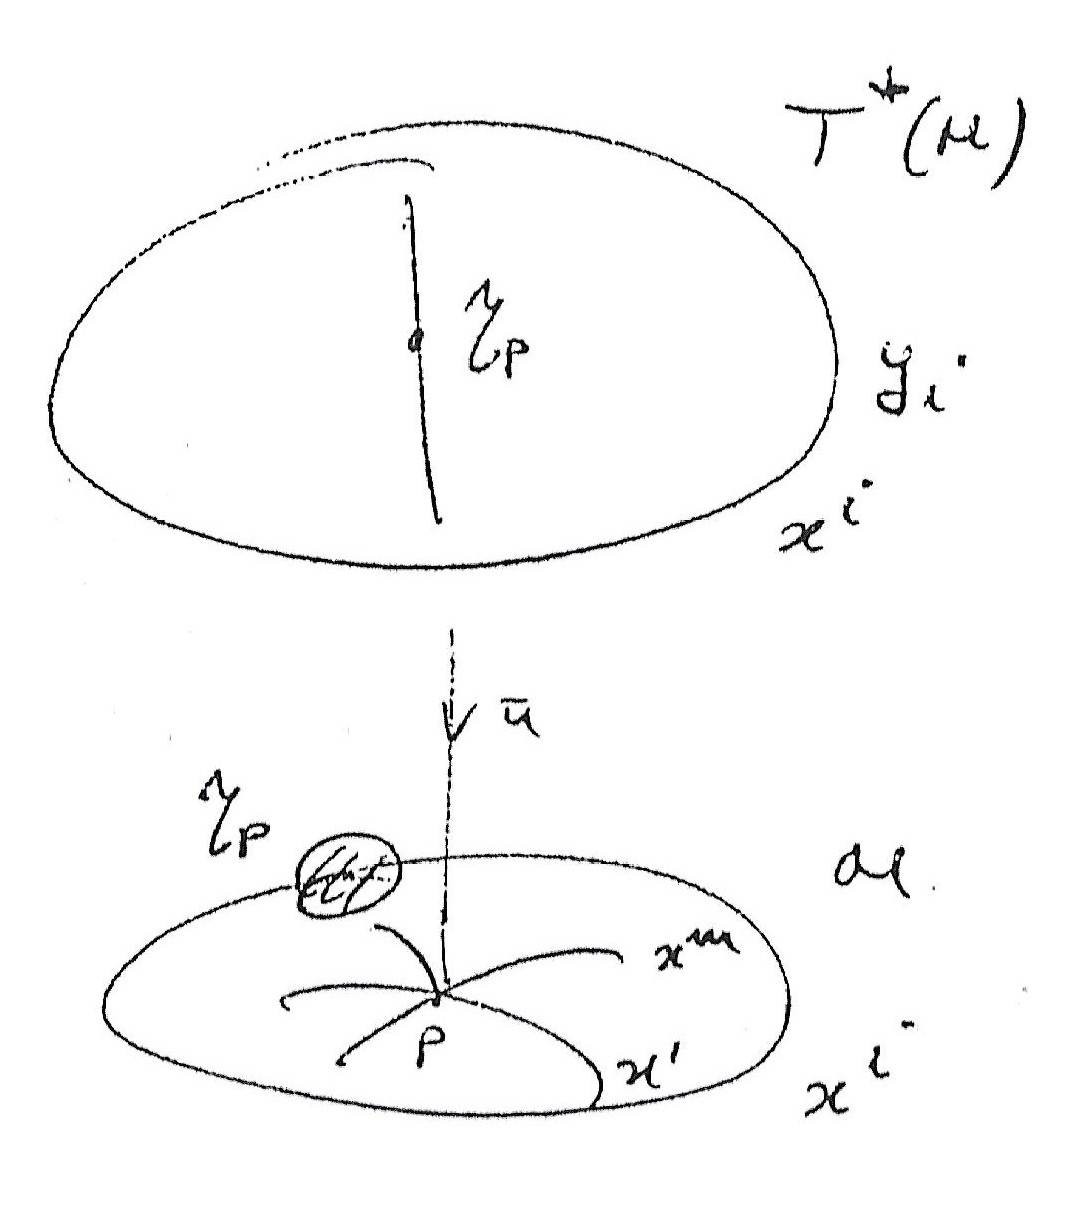
\includegraphics[width=\columnwidth]{media/struttura-simplettica-del-fibrato-cotangente/20-2}
\smallskip
\begin{equation*}
\eta_P = (\eta_P)_i dx^i \overset{def}{=} y_{i_p}(dx^i)_P 
\end{equation*}
\\
$T^*(M) =$ spazio (fibrato su $M$) costituito dalla totalità delle \textit{forme differenziali} applicate in tutti i punti di $M$ \\
$x^i, y_i$ \quad coordinate \textit{naturali} su $T^*(M)$ \\
\begin{equation*}
\eta_P = y_{i_P} dx^i = y_{i_P} \frac{\partial x'}{\partial x'^k} dx'^k 
\end{equation*}
\begin{equation*}
\left\{
\begin{aligned}
x'^i &= x'^i(x^1 \dots x^m) \\
y'^i &= \frac{\partial x^k}{\partial x'^i} (x^1 \dots x^m) y_k \\ 
\end{aligned}
\right.
\end{equation*}
\textit{Trasformazione} tra coordinate \textit{naturali} in $T^* (M)$ \\
\end{multicols}

Concentriamo la nostra attenzione su $ T^* (M) $. Esso ammette i seguenti oggetti invarianti o canonici

\begin{equation*}
\begin{aligned}
\theta &= y_i dx^i &\text{$ 1 $-\textit{forma di Liouville} su } T^* (M) \\
\Omega &= d\theta = dy_i \wedge dx^i &\text{$ 2 $-\textit{forma simplettica} su } T^* (M).
\end{aligned}
\end{equation*}

Per ogni coppia di valori

\begin{equation*}
\begin{aligned}
X &= X^i \frac{\partial}{\partial x^i} + X_i \frac{\partial}{\partial y_i} &\in T (T^* (M)) \\
Y &= Y^i \frac{\partial}{\partial x^i} + Y_i \frac{\partial}{\partial y_i} &\in T (T^* (M))
\end{aligned}
\end{equation*}
l'insieme di $ \Omega $ sulla coppia $ (X, Y) $ è definito da
\begin{equation*}
\Omega(X, Y) = X_i Y^i - X^i Y_i = 
\begin{pmatrix} X^i & X_i \end{pmatrix}
\begin{pmatrix} 0 & -I  \\  I & 0 \end{pmatrix}
\begin{pmatrix} Y^i \\ Y_i \end{pmatrix}
\end{equation*}

dove $ I = \begin{pmatrix} 1 & 0 & \dots \\ 0 & 1 & & \\  \vdots & & \ddots &  \end{pmatrix}_{m \times m}$ \medskip

Si dimostra facilmente, sulla base della legge di trasformazione tra coordinate naturali in $ T^*(M) $ dedotta a pagina precedente, e sulla legge di trasformazione da essa indotta sulle componenti $ X'^i, X'_i, Y'^i, Y'_i $, che $ \Omega (X, Y) \in \mathbb{R} $ risulta \textit{indipendente} dalla scelta delle coordinate, cioè che, introdotte componenti $ X^i, X_i, Y^i, Y_i $ e $ X'^i, X'_i, Y'^i, Y'_i $ dei valori $ X, Y $ nelle diverse coordinate naturali su $ T^* (M) $ si ha che

\begin{equation*}
X'_i Y'^i - X'^i Y'_i = X_i Y^i - X^i Y_i
\end{equation*}

(vedi pagina \pageref{pag:7b_fibr_cot}). \\

% INIZIO PAGINA 21

Il funzionale bilineare $ \Omega(\cdot,\cdot) $ \label{pag:7_fibr_cot} definisce un prodotto scalare (antisimmetrico), e quindi stabilisce una identificazione tra \textit{vettori} (= vettori \textit{controvarianti}) e \textit{forme differenziali} (= vettori \textit{covarianti}) definiti su $T^* (M)$. \\

Posto $ \omega = a_idx^i + b^idy_i \quad \in T^*(T^*(M)) $, il vettore ad esso associato risulta essere

\begin{equation*}
X_\omega = - b^i\frac{\partial}{\partial x^i} + a_i \frac{\partial}{\partial y_i} \quad \in T (T^* (M))
\end{equation*}

come facilmente si può verificare dalla definizione

\begin{equation*}
\langle \omega, Y \rangle = \Omega (X_\omega, Y) \qquad \forall \, Y \in T (T^* (M))
\end{equation*}

\newpage

\begin{multicols}{2}
%\begin{wrapfloat}{figure}{l}{0pt}
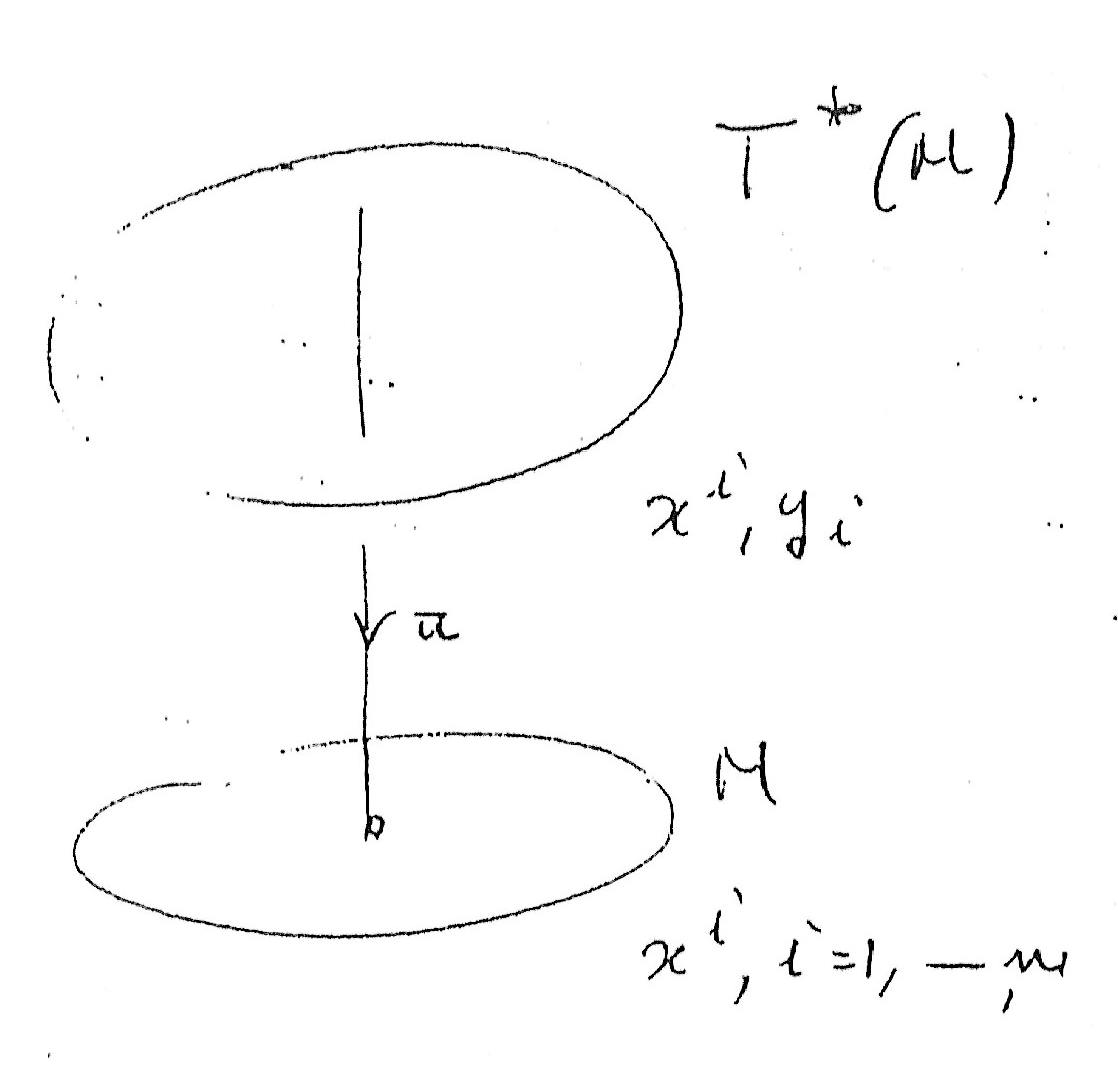
\includegraphics[width=\columnwidth]{media/struttura-simplettica-del-fibrato-cotangente/21-1.jpeg}
%\caption{Esempio di figura ‘‘avvolta’’ da un testo.}
%\end{wrapfloat}
\bigskip
\bigskip
\begin{equation*}
\eta_p \in T_p^* (M) \qquad \eta_p = y_i (dx^i)_p 
\end{equation*}
$ x^i, y_i $ coordinate \textit{``naturali''} in $T^*(M)$
\end{multicols}

Trasformazione tra coordinate naturali $ (x^i, y_i) \rightarrow (x'^i, y'_i) $ in $ T^* (M) $: 
\begin{equation*}
\left \{
\begin{aligned}
&x'^i = x'^i(x^1, \dots x^m) \quad \Leftrightarrow \quad x^k = x^k(x'^1, \dots x'^m) \\
&y'_i = \frac{\partial x^k}{\partial x'^i} (x^1, \dots x^m)y_k 
\end{aligned}
\right.
\end{equation*}

Sia $ X $ un campo vettoriale definito su $ T^* (M) $

\begin{equation*}
X = X^i \frac{\partial}{\partial x^i} + X_i\frac{\partial}{\partial y_i}
\end{equation*}

\begin{equation*}
\begin{aligned}
X &= X^i \bigg( \frac{\partial x'^k}{\partial x^i}\frac{\partial}{\partial x'^k} + \frac{\partial y'_k}{\partial x^i}\frac{\partial}{\partial y'_k} \bigg) + X_i \bigg( \frac{\partial x'^k}{\partial y_i}\frac{\partial}{\partial x'^k} + \frac{\partial y'_k}{\partial y_i}\frac{\partial}{\partial y'_k} \bigg) \\
&= X^i \frac{\partial x'^k}{\partial x^i}\frac{\partial}{\partial x'^k} + X^i \frac{\partial}{\partial x^i} \bigg( \frac{\partial x^r(x')}{\partial x'^k}y_r \bigg) \frac{\partial}{\partial y'_k} + X_i\frac{\partial x^i(x')}{\partial x'^k}\frac{\partial}{\partial y'_k} \\
&= X^i \frac{\partial x'^k}{\partial x^i}\frac{\partial}{\partial x'^k} + X^i \frac{\partial x'^s}{\partial x^i}\frac{\partial}{\partial x'^s} \frac{\partial x^r(x')}{\partial x'^k}y_r\frac{\partial}{\partial y'_k} + X_i\frac{\partial x^i(x')}{\partial x'^k}\frac{\partial}{\partial y'_k} \\
&= X^i \frac{\partial x'^k}{\partial x^i}\frac{\partial}{\partial x'^k} + \bigg( X^i \frac{\partial x'^s}{\partial x^i}\frac{\partial}{\partial x'^s} \frac{\partial x^r(x')}{\partial x'^k}y_r + X_i\frac{\partial x^i(x')}{\partial x'^k} \bigg) \frac{\partial}{\partial y'_k} \\
&\overset{def}{=} X'^k\frac{\partial}{\partial x'^k} + X'_k\frac{\partial}{\partial y'_k}
\end{aligned}
\end{equation*}

con

% INIZIO PAGINA 22

\begin{equation} \label{eq:strutt_fibr_cot_1}
\left\{
\begin{aligned}
X'^k &=: X^i \frac{\partial x'^k}{\partial x^i} \\
X'_k &=: X^i \frac{\partial x'^s}{\partial x^i}\frac{\partial}{\partial x'^s} \frac{\partial x^r(x')}{\partial x'^k}y_r + X_i\frac{\partial x^i(x')}{\partial x'^k}
\end{aligned}
\right.
\end{equation}

Riepilogando, sia $ (x^i, y_i) $ un sistema di coordinate \textit{naturali} su $T^*(M)$, e sia $ (x'^i, y'_i) $ un altro sistema di coordinate \textit{naturali}. Un campo vettoriale $X$ su $T^*(M)$ sarà rappresentato equivalentemente nella forma:
\begin{equation*}
X = X^i \frac{\partial}{\partial x^i} + X_i\frac{\partial}{\partial y_i} = X'^i\frac{\partial}{\partial x'^i} + X'_i\frac{\partial}{\partial y'_i}
\end{equation*}
e il legame tra le componenti $(X^i,X_i)$ e $(X'^i,X'_i)$ nei due sistemi di coordinate è dato dalla formula ($ \ref{eq:strutt_fibr_cot_1} $).\\
Consideriamo ora due campi
\begin{equation*}
\left.X=~\bigg\langle~
\begin{aligned} 
&X^i \frac{\partial}{\partial x^i} + X_i\frac{\partial}{\partial y_i} \\
&X'^i\frac{\partial}{\partial x'^i} + X'_i\frac{\partial}{\partial y'_i}
\end{aligned}
\qquad
\right.Y=~\bigg\langle~
\begin{aligned} 
&Y^i \frac{\partial}{\partial x^i} + Y_i\frac{\partial}{\partial y_i} \\
&Y'^i\frac{\partial}{\partial x'^i} + Y'_i\frac{\partial}{\partial y'_i}
\end{aligned}
\end{equation*}
e il funzionale bilineare (antisimmetrico) definito in coordinate naturali da:
\begin{equation*}
\Omega(X,Y) = X_kY^k - X^kY_k
\end{equation*} 
Mostriamo che la definizione sopra data è \textit{intrinseca}, cioè non dipende dalla scelta delle coordinate, ovvero notiamo che \label{pag:7b_fibr_cot}
\begin{equation*}
X'_kY'^k - X'^kY'_k = X_kY^k - X^kY_k
\end{equation*}
in ogni sistema di coordinate naturali.
\begin{equation*}
\begin{split}
X'_k Y'^k - X'^k Y'_k &= \\
&= \bigg( X^i \frac{\partial x'^s(x)}{\partial x^i}\frac{\partial^2 x^r(x')}{\partial x'^s \partial x'k}y_r + X^i \frac{\partial x^i(x')}{\partial x'^k} \bigg) Y^j\frac{\partial x'^k(x)}{\partial x^j} + \\ 
&\quad - X^i\frac{\partial x'^k(x)}{\partial x^i} \bigg(Y^j \frac{\partial x'^s(x)}{\partial x^i}\frac{\partial^2 x^r(x')}{\partial x'^s \partial x'k}y_r + X^i \frac{\partial x^i(x')}{\partial x'^k} \bigg) \\
&= X^i Y^j \frac{\partial x'^k(x)}{\partial x^j}\frac{\partial^2 x^r(x')}{\partial x'^s \partial x'k}\frac{\partial x'^s(x)}{\partial x^i}y_r + X_i Y^j \frac{\partial x^i(x')}{\partial x'^k}\frac{\partial x'^k(x)}{\partial x^j} + \\ 
&\quad - X^iY^j \frac{\partial x'^k(x)}{\partial x^i}\frac{\partial^2 x^r(x')}{\partial x'^s \partial x'k}\frac{\partial x'^s(x)}{\partial x^i}y_r - X^i Y_j \frac{\partial x'^k(x)}{\partial x^i}\frac{\partial x^j(x')}{\partial x'^k} \\
&= X^i Y^j \frac{\partial x'^s(x)}{\partial x^i}y_r + X_i Y^j - X^i Y^j \frac{\partial x'^s(x)}{\partial x^i}y_r - X^i Y_j \\
&= X_i Y^j - X^i Y_j
\end{split}
\end{equation*}
